Dans le magasin d'Hugo, les clients peuvent louer deux types de vélos : vélos de route ou bien vélos tout terrain. 

Chaque type de vélo peut être loué dans sa version électrique ou non.

On choisit un client du magasin au hasard, et on admet que :
%
\begin{itemize}
	\item Si le client loue un vélo de route, la probabilité que ce soit un vélo électrique est de 0,4 ;
	\item Si le client loue un vélo tout terrain, la probabilité que ce soit un vélo électrique est de 0,7 ; \item La probabilité que le client loue un vélo électrique est de 0,58.
\end{itemize}
%
On appelle $\alpha$ la probabilité que le client loue un vélo de route, avec $0 \leqslant \alpha \leqslant 1$. 

On considère les évènements suivants:

\begin{itemize}
	\item $R$ : \og le client loue un vélo de route \fg{} ;
	\item $E$ : \og le client loue un vélo électrique \fg{} ;
	\item $\overline{R}$ et $\overline{E}$ , évènements contraires de $R$ et $E$.
\end{itemize}

\begin{wrapstuff}[r,leftsep=1.5em,rightsep=1em,abovesep=0pt,belowsep=0pt]
	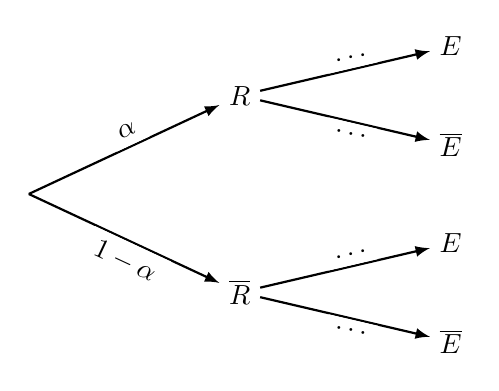
\begin{tikzpicture}[xscale=1,yscale=1]
		\tikzstyle{fleche}=[->,>=latex,thick]
		\tikzstyle{noeud}=[]
		\tikzstyle{etiquette}=[pos=0.55,sloped,fill=white]
		\def\DistanceInterNiveaux{2.33}
		\def\DistanceInterFeuilles{1}
		\def\NiveauA{(0)*\DistanceInterNiveaux}
		\def\NiveauB{(1.15)*\DistanceInterNiveaux}
		\def\NiveauC{(2.3)*\DistanceInterNiveaux}
		\def\InterFeuilles{(-1.25)*\DistanceInterFeuilles}
		\coordinate (R) at ({\NiveauA},{(1.5)*\InterFeuilles}) ;
		\node[noeud] (Ra) at ({\NiveauB},{(0.5)*\InterFeuilles}) {$R$};
		\node[noeud] (Raa) at ({\NiveauC},{(0)*\InterFeuilles}) {$E$};
		\node[noeud] (Rab) at ({\NiveauC},{(1)*\InterFeuilles}) {$\overline{E}$};
		\node[noeud] (Rb) at ({\NiveauB},{(2.5)*\InterFeuilles}) {$\overline{R}$};
		\node[noeud] (Rba) at ({\NiveauC},{(2)*\InterFeuilles}) {$E$};
		\node[noeud] (Rbb) at ({\NiveauC},{(3)*\InterFeuilles}) {$\overline{E}$};
		\draw[fleche] (R)--(Ra) node[etiquette,above] {$\alpha$};
		\draw[fleche] (Ra)--(Raa) node[etiquette,above] {$\ldots$};
		\draw[fleche] (Ra)--(Rab) node[etiquette,below] {$\ldots$};
		\draw[fleche] (R)--(Rb) node[etiquette,below] {$1-\alpha$};
		\draw[fleche] (Rb)--(Rba) node[etiquette,above] {$\ldots$};
		\draw[fleche] (Rb)--(Rbb) node[etiquette,below] {$\ldots$};
	\end{tikzpicture}
\end{wrapstuff}
%
On modélise cette situation aléatoire à l'aide de l'arbre reproduit ci-contre :

Si $F$ désigne un évènement quelconque, on notera $p(F)$ la probabilité de $F$.

\begin{enumerate}
	\item Recopier cet arbre sur la copie et le compléter.
	\item 
	\begin{enumerate}
		\item Montrer que $p(E) = 0,7 - 0,3\alpha$.
		\item En déduire que : $\alpha = 0,4$.
	\end{enumerate}
	\item On sait que le client a loué un vélo électrique. 
	
	Déterminer la probabilité qu'il ait loué un vélo tout terrain. On donnera le résultat arrondi au centième.
	\item Quelle est la probabilité que le client loue un vélo tout terrain électrique ?
	\item Le prix de la location à la journée d'un vélo de route non électrique est de $25$ euros, celui d'un vélo tout terrain non électrique de $35$~euros. 
	
	Pour chaque type de vélo, le choix de la version électrique augmente le prix de location à la journée de $15$~euros. 
	
	On appelle $X$ la variable aléatoire modélisant le prix de location d'un vélo à la journée. 
	\begin{enumerate}
		\item Donner la loi de probabilité de $X$. On présentera les résultats sous forme d'un tableau.
		\item Calculer l'espérance mathématique de $X $et interpréter ce résultat.
	\end{enumerate}	
	\item Lorsqu'on choisit $30$ clients d'Hugo au hasard, on assimile ce choix à un tirage avec remise. 
	
	On note $Y$ la variable aléatoire associant à un échantillon de 30 clients choisis au hasard le nombre de clients qui louent un vélo électrique.
	
	On rappelle que la probabilité de l'événement $E$ est : $p(E) = 0,58$.
	\begin{enumerate}
		\item Justifier que $Y$ suit une loi binomiale dont on précisera les paramètres.
		\item Déterminer la probabilité qu'un échantillon contienne exactement $20$ clients qui louent un vélo électrique. On donnera le résultat arrondi au millième.
		\item Déterminer la probabilité qu'un échantillon contienne au moins $15$ clients qui louent un vélo électrique. On donnera le résultat arrondi au millième.
	\end{enumerate}
\end{enumerate}

